
In several contexts, the functional data are contamined with noise.
This contamination can be due to errors in the measure procedure or to
the intrinsic random behaviour of the process,
this will motivate the use of smoothing splines.

\begin{figure}[Example of smoothing]{FIG:SMOOTHING}{Smoothing interpolation}
	\subfigure[SBFIG:SMOOTHING1]{Cubic smoothing}{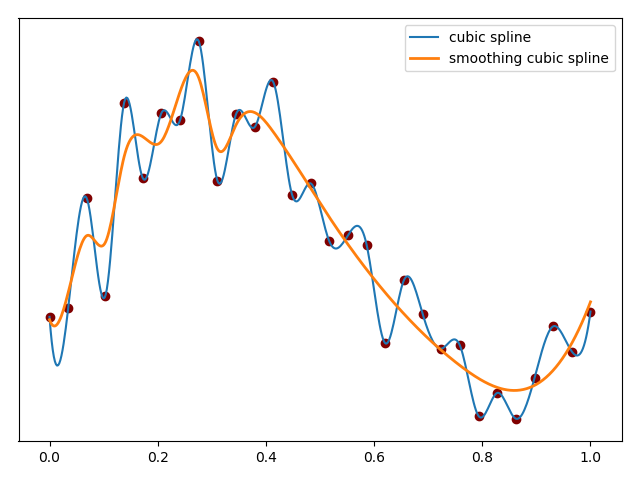
\includegraphics[width=7.5cm]{smoothing-splines}} \quad
	\subfigure[SBFIG:SMOOTHING2]{Several values of the smoothing factor}{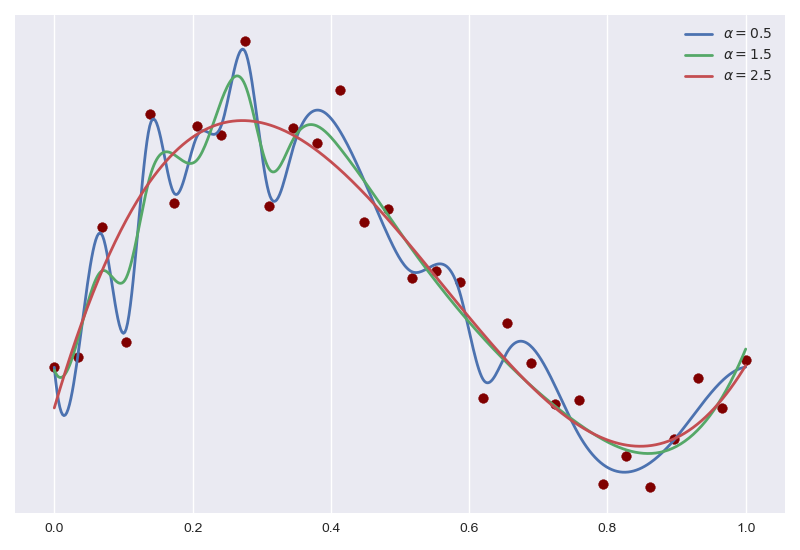
\includegraphics[width=7.5cm]{smoothing-splines-values}}
\end{figure}

This method is a variant of the spline interpolation, but we will not
use directly the points $\{t_k\}_{k=1}^{N}$ as knots. Instead, we will use a
smaller set of knots $\{\tilde t_k\}_{k=1}^{M}$, generally different from the
originals, with their corresponding values $\tilde y_k = f(\tilde t_k)$
calculated using spline interpolation. The function interpolated using smoothing
splines will be defined using spline interpolation on the set of knots
$(\tilde t_k, \tilde y_k)$. Figure \ref{FIG:SMOOTHING} shows the smoothing
interpolation of a noisy observation.

To determine the knots $\tilde t_k$ is used an smoothing parameter $\alpha$.
A weight $w_k$ is assigned to each of the original points $t_k$, used to calculate
the knots $\tilde t_k$ as a weighted average of the original ones. These weights
can be set uniformly.
The number of knows will be increased until the smoothing condition is satisfied,
defined as

\begin{equation}[]{Smoothing condition}
\sum_{k=1}^N \left (  w_k (y_k - \tilde f(t_k)) \right)^2 \le \alpha
\end{equation}

where $\tilde f(t_k)$ is the value of the smoothing spline at $t_k$.
In other words, the smoothing parameter sets the maximum value of the residuals.

After representing the data as continuous functions, we can move on to other
parts of the analysis, such as the study of variability due to the continuous
structure of the data, called registration of the data. The techniques used
during the registration of the data require the use of a discrete
representation of the functions and their evaluation in arbitrary points,
which is done by interpolation.
